\begin{corr}{Champ électrique dans les conducteurs}
	\correction{Effet de peau}
	\begin{corrlist}
		\item Une exponentielle est sans dimension, \fbox{$j_0$ s'exprime donc en 
			$\ampere \usk \rpsquare \meter$.}
			L'argument à l'intérieur d'une fonction est toujours sans
			dimension. \fbox{$\delta$ est donc homogène à une longueur.}
			La fonction $\exp\left(-\dfrac{x}{\delta}\right)$
			tend rapidement vers $0$. $\delta$ correspond donc à la
			profondeur de pénétration de $\vecj$, et donc de 
			l'onde électromagnétique, dans le conducteur.
		\item $\omega$ s'exprime en $\rad \usk \reciprocal \second$ et  
		  $\sigma$ s'exprime en $S \usk \reciprocal \meter$, c'est-à-dire 
		  en $\ampere \squared \usk \cubic \second \usk \reciprocal \kilogram
		  \usk \rpcubic \meter$. Le radian est une "fausse" unité car il
		  correspond au rapport de deux longueurs. Le produit $\mu_0
		  \omega \sigma$ est donc homogène à l'inverse du carré d'une longueur.
		  $\delta$ est donc bien homogène à une longueur.
		\item  On cherche à savoir ici si l'onde électromagnétique
		   plonge assez loin dans le sol pour atteindre le gisement de 
		   pyrrhotite. L'épaisseur de peau vaut dans les deux cas
		   \begin{corrlist}
			   \item $\sqrt{\dfrac{2 \times 100}{4 \pi \times 10^{-7} 
			    \times 1 \times 10^3 \times 2\pi}}
			  = \unit{0.16}{\kilo \meter}$
			\item $\sqrt{\dfrac{2 \times 100}{4 \pi \times 10^{-7} 
			    \times 1 \times 10^8 \times 2\pi}}
			  = \unit{50}{\centi \meter}$
		  \end{corrlist}
		  Le radar ne permettrait donc pas de détecter le gisement.

   	\item Pour le cuivre à température ambiante, $\sigma \approx 
          \unit{5.9 \times 10^7}{\siemens \usk \reciprocal \meter}$. 
	  Dans ce cas, $\delta \approx \unit{10}{\nano \meter}$, expliquant ainsi
	  l'opacité du cuivre.
	\end{corrlist}


\correction{Contamination d'un aquifère}
	\begin{corrlist}
		\item Voir figure~\ref{fig:aquiferes_corr}a.
		\item \fbox{On distingue deux couches de résistivités respectives 
		  $\rho_1 = \unit{29.0}{\ohm \usk \meter}$ et $\rho_2 =
	  \unit{6.4}{\ohm \usk \meter}$.} L'eau salée a une résistivité plus faible
		  que l'eau douce. La couche la plus profonde correspond donc à l'eau salée.
		\item Dans notre exercice, $k \approx -0.6$. La courbe qui nous intéresse
		  est donc celle possédant le même $k$ dans la 
		  figure~\ref{fig:aquiferes}. Cette courbe passe notamment 
		  par le point $(2, 0.5)$. Pour déterminer la profondeur de 
		  l'interface eau douce - eau salée, on trace la résistivité apparente
		  normalisée en fonction de la distance inter-électrodes normalisée
		  pour différentes valeur de $d$ (voir Fig.~\ref{fig:aquiferes_corr}b).
		  \fbox{On en déduit que $d$ est ici de l'ordre de $\unit{100}{\meter}$.}
	\end{corrlist}


\begin{figure}[h!]
	\centering
	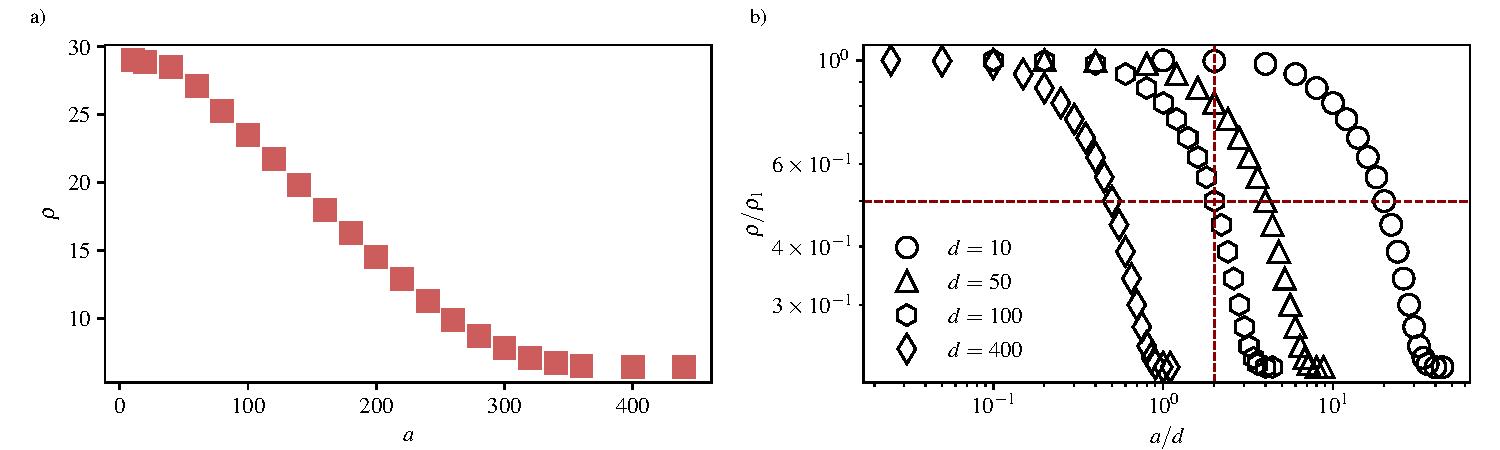
\includegraphics[width=0.8\linewidth]{aquiferes_corr}
	\caption{Résistivité apparente $\rho$ mesurée en fonction de la distance
	         inter-électrodes $a$ à gauche. Résistivité apparente normalisée
	 	 par la résistivité de la couche $1$ en fonction de la distance 
	 	inter-électrodes normalisée par l'épaisseur de la couche $1$
		à droite pour différentes valeurs de $d$. Sur le panel de 
		droite, les lignes en tiret se croisent au point $(2, 0.5)$.}%
	\label{fig:aquiferes_corr}
\end{figure}

\correction{Le condensateur plan}
\begin{corrlist}
	\item Voir la figure.~\ref{fig:condensateur}
	\item Nous savons que le champ électrostatique $\vece$ est lié au potentiel
	      électrostatique $V$ par la relation
	      \begin{equation*}
		      \vece = - \grad(V).
	      \end{equation*}
	      Le champ électrique est donc dirigé des potentiels les plus élevés 
	      aux potentiels les plus faibles. La plaque $1$ étant chargée positivement
	      et la plaque $2$ négativement, \fbox{$\vece$ en un point situé à l'intérieur des
      plaques est dirigé de la plaque $1$ à la plaque $2$.}
      \item Dans un repère cartésien, la forme générale du champ électrique $\vece$ 
	    en un point $M$ de l'espace de coordonnée $(x, y, z)$ est la suivante
	    \begin{equation*}
		    \vece(M) = E_x(x, y, z)\ex + E_y(x, y, z)\ey + E_z(x, y, z)\ez.
	    \end{equation*}
	    Pour simplifier cette expression, on commence par étudier les invariances de la
	    distribution de charge générant le champ électrique $\vece$
	    \begin{itemize}
		    \item les deux plaques étant infinies, le système est invariant
			  par translation selon l'axe $\ez$. $\vece$ ne dépend pas
			  de $z$,
		    \item le système est invariant par translation selon $\ey$.
			  $\vece$ ne dépend pas de $y$.
	   \end{itemize}
	   \fbox{$\vece$ ne dépend donc que de $x$}.

	   On étudie maintenant les symétries de cette distribution de charge 
	   en considérant un point $M$ quelconque de l'espace
	   \begin{itemize}
		   \item le plan $(M, \ex, \ey)$ est un plan de symétrie de 
			 la distribution de charges. $\vece(M)$ doit donc
			 appartenir à ce plan,
		   \item le plan $(M, \ex, \ez)$ est un plan de symétrie de la
			 distribution de charge. $\vece(M)$ doit donc appartenir
			 à ce plan.
	 \end{itemize}
	 $\vece(M)$ doit appartenir aux plans $(M, \ex, \ey)$ et $(M, \ex, \ez)$, 
	 \fbox{il est donc colinéaire à $\ex$}. On a finalement
	 \begin{equation}
		 \vece(M) = E(x)\ex,
	 \end{equation}
	 en tout point de l'espace $M$. Cette forme simple est propice à 
	 l'utilisation du théorème de Gauss.

 	 \item On applique donc le théorème de Gauss aux trois surfaces fermées
	       proposées
	       \begin{corrlist}
		       \item La surface fermée ne contient aucune charge, le flux
			     de $E$ à travers cette surface est donc nul. On a donc
			     $E(a_1) = E(a_2)$. Comme nous n'avons imposé aucune condition
			     sur le placement de la surface (hormis le fait
			     qu'elle soit incluse entre les deux plaques), on peut
			     conclure que \fbox{$\vece$ est uniforme entre les deux plaques.}
		       \item Par un raisonnement analogue, on conclut que $\vece$
			     est uniforme à l'extérieur des plaques. \fbox{$\vece$ doit
			     donc être nul à l'extérieur des plaques} pour éviter la génération
		     par ce système d'une énergie infinie.
	     		\item La surface contient la charge $\sigma S$. Le théorème de
			Gauss donne donc
			\begin{equation*}
			E(b_1) - E(b_2) = \dfrac{\sigma}{\epsilon_0}.
			\end{equation*}
			$E(b_2)$ étant nul on obtient finalement
			\begin{equation*}
				E(b_1) = \dfrac{\sigma}{\epsilon_0}
			\end{equation*}
			\begin{defn}[Relation de continuité du champ électrostatique]
				Au passage d'une surface possédant une densité surfacique de
				charge $\sigma$, 
				\begin{itemize}
					\item la composante du champ électrostatique
					      $\vece$ tangentielle à la surface est
					      conservée,
					 \item la composante normale à la surface est 
					       discontinue. Cette discontinuité vaut
					       \begin{equation}
						       \Delta E = \dfrac{\sigma}{\epsilon_0}
					       \end{equation}
			      \end{itemize}
			\end{defn}
			Finalement,
			\begin{itemize}
				\item \fbox{Le champ électrique est uniforme entre les
				  deux plaques et vaut 
			          $\vece = \dfrac{\sigma}{\epsilon_0}\ex$.}
				\item \fbox{Le champ électrique est nul en dehors des
					plaques.}
		      \end{itemize}
	       \end{corrlist}
\end{corrlist}

\begin{figure}[h]
	\centering
	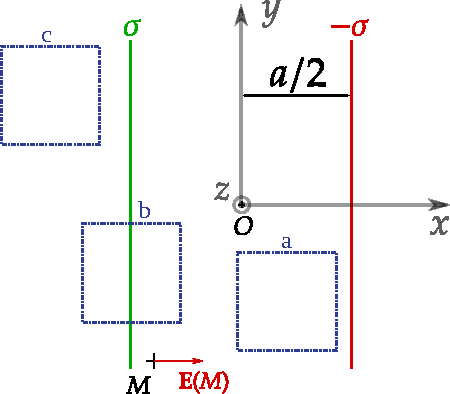
\includegraphics[scale=0.8]{condensateur}
	\caption{Condensateur plan composé d'une plaque chargée positivement avec 
	         une densité surfacique de charge $\sigma$ et une plaque chargée
	 	 négativement avec une densité surfacique de charge $-\sigma$.}%
	\label{fig:condensateur}
\end{figure}
\end{corr}
